\documentclass{standalone}
\usepackage{tikz}
\usepackage{varwidth}

\begin{document}
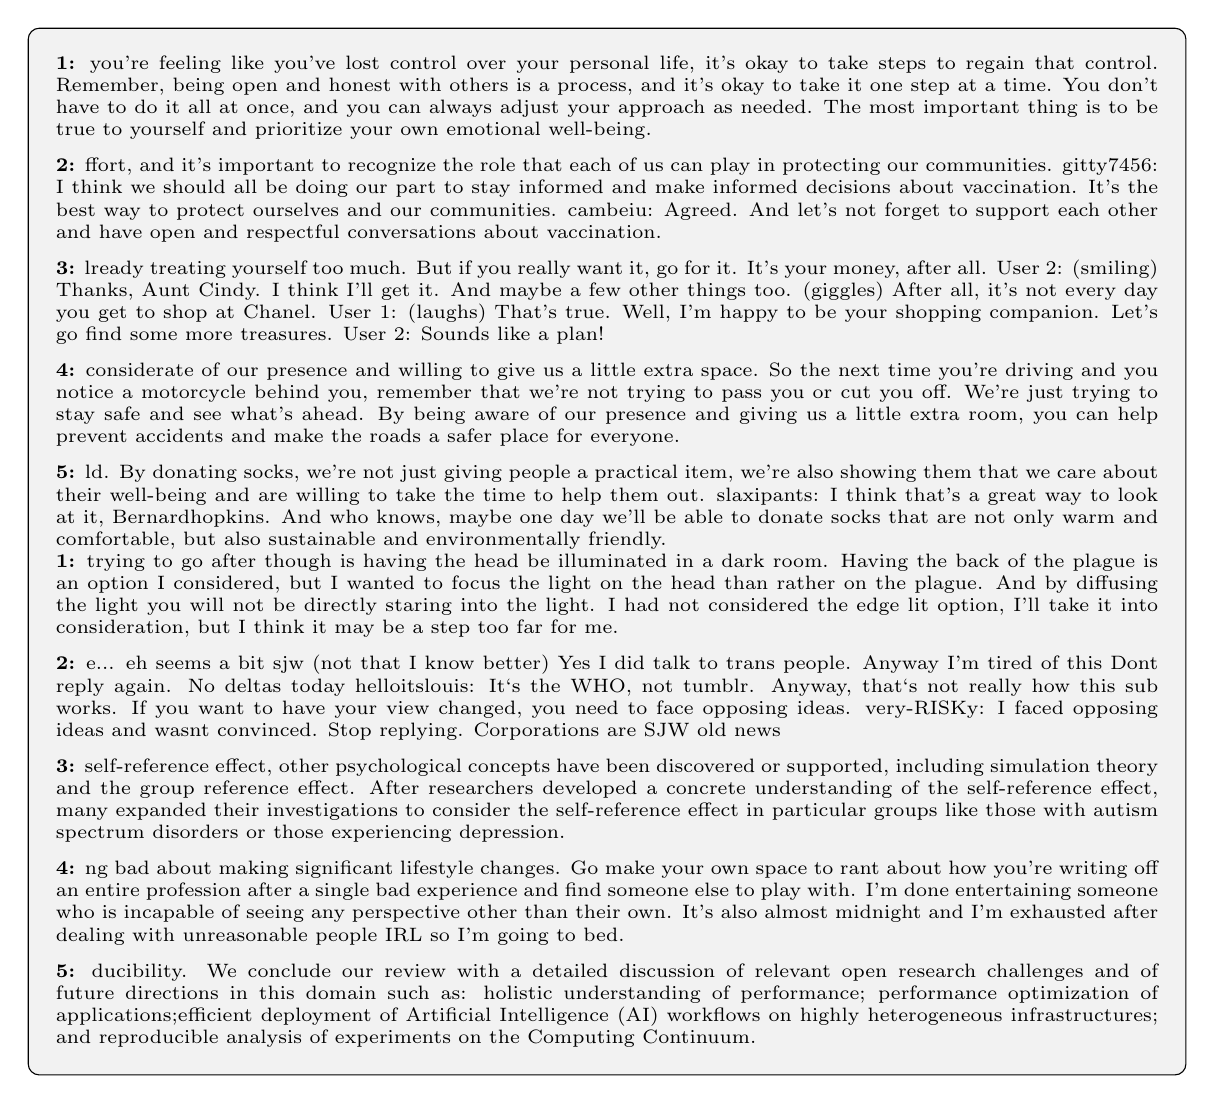
\begin{tikzpicture}
    % Box with adjusted margins and formatting
    \node[draw, fill=gray!10, text width=14cm, align=justify, inner sep=10pt, rounded corners, font=\scriptsize] (box) {
        \textbf{1:} you're feeling like you've lost control over your personal life, it's okay to take steps to regain that control.
Remember, being open and honest with others is a process, and it's okay to take it one step at a time. You don't have to do it all at once, and you can always adjust your approach as needed. The most important thing is to be true to yourself and prioritize your own emotional well-being.\\[5pt]
        \textbf{2:} ffort, and it's important to recognize the role that each of us can play in protecting our communities.
gitty7456: I think we should all be doing our part to stay informed and make informed decisions about vaccination. It's the best way to protect ourselves and our communities.
cambeiu: Agreed. And let's not forget to support each other and have open and respectful conversations about vaccination.\\[5pt]
        \textbf{3:} lready treating yourself too much. But if you really want it, go for it. It's your money, after all.
User 2: (smiling) Thanks, Aunt Cindy. I think I'll get it. And maybe a few other things too. (giggles) After all, it's not every day you get to shop at Chanel.
User 1: (laughs) That's true. Well, I'm happy to be your shopping companion. Let's go find some more treasures.
User 2: Sounds like a plan!\\[5pt]
        \textbf{4:} considerate of our presence and willing to give us a little extra space.
So the next time you're driving and you notice a motorcycle behind you, remember that we're not trying to pass you or cut you off. We're just trying to stay safe and see what's ahead. By being aware of our presence and giving us a little extra room, you can help prevent accidents and make the roads a safer place for everyone.\\[5pt]
        \textbf{5:} ld. By donating socks, we're not just giving people a practical item, we're also showing them that we care about their well-being and are willing to take the time to help them out.
slaxipants: I think that's a great way to look at it, Bernardhopkins. And who knows, maybe one day we'll be able to donate socks that are not only warm and comfortable, but also sustainable and environmentally friendly.
\\
        \textbf{1:} trying to go after though is having the head be illuminated in a dark room. Having the back of the plague is an option I considered, but I wanted to focus the light on the head than rather on the plague. And by diffusing the light you will not be directly staring into the light.
I had not considered the edge lit option, I'll take it into consideration, but I think it may be a step too far for me.\\[5pt]
        \textbf{2:} e... eh seems a bit sjw (not that I know better) 
Yes I did talk to trans people. Anyway I’m tired of this Dont reply again. No deltas today
helloitslouis: It‘s the WHO, not tumblr.
Anyway, that‘s not really how this sub works. If you want to have your view changed, you need to face opposing ideas.
very-RISKy: I faced opposing ideas and wasnt convinced. Stop replying. Corporations are SJW old news\\[5pt]
        \textbf{3:} self-reference effect, other psychological concepts have been discovered or supported, including simulation theory and the group reference effect.
After researchers developed a concrete understanding of the self-reference effect, many expanded their investigations to consider the self-reference effect in particular groups like those with autism spectrum disorders or those experiencing depression.\\[5pt]
        \textbf{4:} ng bad about making significant lifestyle changes.
Go make your own space to rant about how you're writing off an entire profession after a single bad experience and find someone else to play with. I'm done entertaining someone who is incapable of seeing any perspective other than their own.
It's also almost midnight and I'm exhausted after dealing with unreasonable people IRL so I'm going to bed.\\[5pt]
        \textbf{5:} ducibility. We conclude our review with a detailed discussion of relevant open research challenges and of future directions in this domain such as: holistic understanding of performance; performance optimization of applications;efficient deployment of Artificial Intelligence (AI) workflows on highly heterogeneous infrastructures; and reproducible analysis of experiments on the Computing Continuum.
    };
\end{tikzpicture}
\end{document}
